\chapter{Theoretical Background}
\label{chapter:Theoretical Background}
%\textit{The chapter presents the theories and models that underpin the research study. It explains the concepts and theoretical approaches that will guide the analysis.} \\
%\textit{The framework ensures a description of the geohydrologicalal and ecohydrologicalal system of Rotterdam, which accommodates a base for this research study. Continuing with subsections regarding groundwater level collection and monitoring in the Netherlands. The chapter ends with a subsection regarding the current groundwater management and policies on national and regional scale.}
%Within the municipal area of Rotterdam, the included neighborhoods are: 
%Charlois, Delfshaven, Feijenoord, Hillegersberg-Schiebroek, Hoogvliet, Hoek van Holland, %IJsselmonde, Kralingen-Crooswijk, Noord, Overschie, Prins Alexander, Pernis, Rozenburg, %Rotterdam Centrum, Rotterdam Noord-West.


\section{System description}
A system description can be regarded as the verbal model of distinguishable hydrological systems, as they influence nature reserves \cite{ganswijk-1988}. Next to the hydrological system, the geological and ecological system will also be included. A system description can be built according to: 1) The description of the local geohydrological system; 2) The description of the regional geohydrological system; 3) The interaction between the local and regional system; 4) The relationship between the groundwater and surface water system \cite{koomen-2011}. As well as the quantity and quality aspects of the area. Within the system description, emphasis lies on particle and water flow as a function of time and place to the root zone of valuable habitats \cite{ganswijk-1988}. 

\subsection{Geohydrological system description}
To start with the geological formations within the municipal boundaries. Throughout the municipal area, the formation is complex \cite{valstar-2019}. Meaning that there are strongly heterogeneous formations with local gully erosion and cuts. A heterogeneous formation refers to geological layers that differ in parameters as structure, composition, density, and permeability \cite{valstar-2019}. The subsoil mainly consists of clay and sandy soils, the distinction is made regarding the permeability of the soils. The presence of creeks has influenced the erosion of peat and sandy channel depositions, resulting in the creation of levees \cite{janssen-2005}. By the influence of wind throughout the municipal area, river dunes advanced along old river courses. River dunes and levees form sand channels and ensure different groundwater flows. 
The municipal area of Rotterdam is located in the western part of the Dutch delta. Over the past 10.000 years, the area has been influenced by the North Sea. This can be seen through a layer of 20 meters of mudflat and lagoon deposits from the Holocene period. While the mudflat deposits consist of sand, silt, and clay, the lagoon deposits consist of silt, clay, and peat. Because of the influence of the North Sea, there is much spatial variation in the Holocene cover layer. Previous intrusions of the North Sea within the municipal area resulted in a boundary between fresh and salt groundwater that is found in the upper part of the Holocene layer. The distribution of fresh water and salt water is also influenced by water management, for example land reclamation of polder areas and water abstraction. The morphology of the municipal area is influenced by the presence of the river Meuse, the large scale embankment and excavation of the port and industrial area. Rivers in the lower polder area that are located within the dike ring, cross the polder areas and characterize the groundwater flow situation in Rotterdam. Seepage from the river mainly infiltrates into the first aquifer. River water from the first aquifer occurs as seepage into the lower polder areas. The infiltrating river water flows into the deeper aquifers or is caught for other purposes such as industry \cite{janssen-2005}. \\
\begin{figure}[htbp]
    \centering
    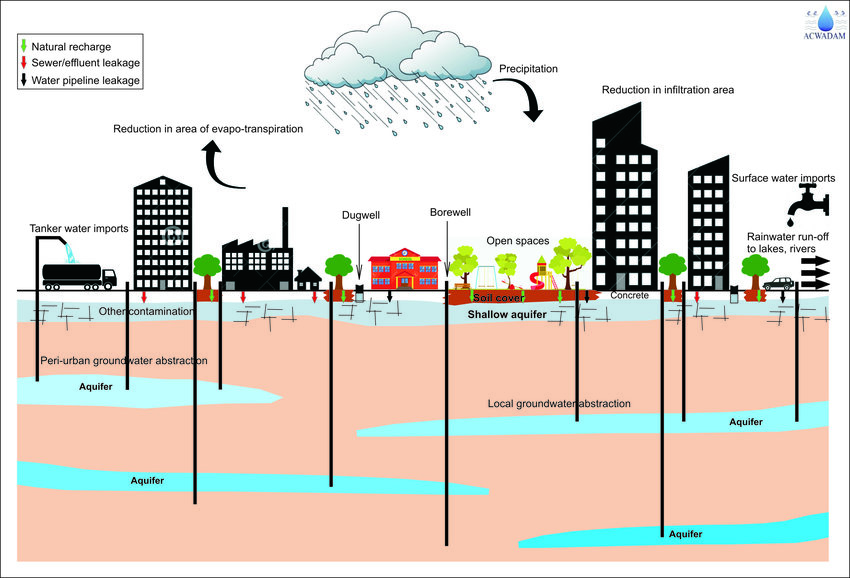
\includegraphics[width=0.95\linewidth]{figures/figures theory/urbanflow.png}
    \caption{Regional groundwater flow in urban areas \cite{siddique-2017}.}
    \label{gwflow}
\end{figure}
\\
As shown in figure \labelcref{gwflow}, the top-soil layer is influenced by human interventions. Consequently, the top-soil layer, or also called the Anthropocene layer, varies in soil composition. The distribution of the top layer is derived from the height of the ground level and top layer of the Holocene cover layer. Underneath the Holocene phreatic package, the overburden layer (Westland) is present. The overburden layer consists of sandy material that is associated with the occurrence of channel fillings or old river dunes, which means that the covering layer has a greater permeability \cite{janssen-2005}. The Holocene overburden is bounded at the bottom by the first Pleistocene aquifer (Twente, Eem, Urk, and Kreftenheye). The layer consists of fine and coarse sands and gravel with intercalations of sand. In the middle of the first aquifer is a compacted peat layer. The aquifer system is thinner in the south than in the north of the municipal area. Below the first aquifer lies a poorly permeable layer (Kedichem and Tegelen) which is formed by a package of sandy clay's with intercalations of sand. In the middle of the permeable layer is a compacted layer of peat. Below the first permeable layer, a second aquifer is present (Tegelen). The second aquifer consists of fine-medium sandy layers with a high permeability. The second aquifer has a thickness of 30-100 meters. An additional second poorly permeable layer (Tegelen) is present between the second and third aquifer (Maassluis). This layer is made of clay deposits and has a varying thickness between 50-100 meters. The third aquifer characterizes itself by fine to medium sandy layers. The thickness of the third aquifer varies from 50-100 meters. The bottom of the geohydrological system (Pliocene: Formation of Oosterhout) consists of impermeable clay deposits. The second and third aquifer systems are thick in the center, but thinner on the eastern and western side of the municipal area \cite{janssen-2005}. As previously mentioned, an additional Anthropocene top layer is supplemented on the top layer of the Holocene deposition. Sand-filled vertical drains are used to add vertical drainage, which can accelerate the discharge of infiltrated water into the deep groundwater. Flow occurs from a high hydraulic head to a low hydraulic head. In this situation, flow might occur from the dunes on the western side of the municipal area to the polders farther inland. Higher lying areas can serve as infiltration areas where groundwater flows through the deeper layers to the deeper polders in addition to the hydraulic head differences that causes groundwater flow \cite{valstar-2019}. Seepage and infiltration patterns can only be considered at regional scale, not at local scale \cite{koomen-2011}. \\
\\
The geological and hydrological complexity of Rotterdam displays a diversity of soil types, but is characterized by sandy soils, clay, and peat. The heterogeneity is a result of depositions of mudflat and lagoon sediments during the Holocene period. Also, erosion and deposition corresponding to ancient river systems and the influence of the North Sea. A landscape is created in which groundwater flow patterns are influenced by the spatial variability in soil type and the corresponding hydraulic properties. Presently, the Anthropocene layer consists of permeable sand and the thickness varies between centimeters to approximately 30 meters at Maasvlakte, at the western side of the municipal area. Within the city, the process of soil consolidation takes place and in order to prevent further consolidation, supplementary sand is added. Through this process, the top layer is strongly affected by Anthropocene influences.  Outside of the road cunet, the soil is more clayey and likely to be less permeable. The geohydrological dynamics, that are influenced by hydraulic properties of the soil types, affect the groundwater system and thus the strategies that are suitable regarding optimal groundwater management \cite{janssen-2005}.

\subsection{Ecohydrological system description}
The interplay between ecology and hydrology can be defined as the effects an ecological system has on the groundwater system. For example: Evapotranspiration from shallow groundwater \cite{ganswijk-1988}. Ecological factors help to define spatial and temporal scales, which are smaller than geohydrological characterizations. Groundwater perceived ecological functions extend beyond encompassing stream flows, moderating water level fluctuations in lakes and wetlands reliant on groundwater resources, enrichment of ecosystems with nutrients, and hydration of riparian zones and groundwater-dependent vegetation.

The main objective for the description of ecohydrology within the municipal area of Rotterdam is in what way the ecohydrological system can be influencing the groundwater system. Important parameters are the overall structure of the study area (urban or rural), the characteristic ecosystems and gradients that are present, the amount of precipitation and evaporation that could influence the groundwater level in the study area. It has to be noted that specific local conditions, species composition, and community structure will not be discussed in this research study \cite{koomen-2011}.\\
\\
Commencing, the municipal area is located next to a rural region filled with grassland that comprises peat meadows and agricultural land. In the western part of the area, a broad coastal zone that consists of dunes, beaches, and forests in the inner dune area are present. The area is characterized by: 1) A transition of high lying peat meadows to reclaimed land; 2) A transition of coastal dunes to beach walls to peat meadows to reclaimed land; 3) A transition of river areas to peat meadows and reclaimed land. Overall, the characteristic ecosystem of the municipal area can be identified as river and brook valleys, coastal dunes, marshes, grass, and arable land in combination with urban development \cite{koomen-2011}. Groundwater and surface waters interact through ecohydrological processes. The groundwater level correlates with the ground level and influences the vegetation composition at local scale. Since the height of the groundwater level influences the oxygen concentration and extent of moisture that is available in the soil, surface waters interchange with nearby groundwater \cite{witte-2008}. 

\section{Hydrological cycle in urban areas}
Urbanisation is a far-reaching process that has influence on the hydrological cycle in an area \cite{bakel-1995}. The hydrological cycle in urban areas is different than the hydrological cycle in rural areas. A key distinction in the cycle among urban and rural landscapes lies in surface sealing and the transport of precipitation through surface runoff. It is proven that the water balance transforms when urbanisation takes place. The effects of urbanisation on the hydrological cycle are: 1) Decrease of evaporation; 2) Decrease of percolation and capillarity, because of a loss in permeable surfaces \cite{etikala-2022}; 3) Decrease of the net groundwater recharge with optional processes as seepage; 4) Increase of discharge to surface waters, because of surface sealing and drainage measures; 5) Discharge to a WWTP.\\
\\
A major element of the hydrological cycle is groundwater recharge as a result of percolation and capillarity. The consequence of urbanisation is the reduction of groundwater recharge, because of surface sealing. Typically, in urban environments, precipitation rarely contributes to groundwater recharge. This is true for heavy rainfall events, during which no time is available to infiltrate into the soil. Conversely, light rainfall events result often in groundwater recharge. \\
\\
Urban areas have a dual hydrological system: A modified natural drainage system and an artificial water supply and wastewater disposal system \cite{douglas-2020}.  Throughout City of Rotterdam, the modified natural drainage system includes canals and river diversions such as the \textit{"Nieuwe Waterweg".}

\section{Collection of groundwater level data}
Measurements of groundwater levels are necessary for understanding subsurface dynamics \cite{hendriks-2023}. This section discusses the practice of groundwater level measurements, types of monitoring wells, and the influence of groundwater flow dynamics on measurements. \\
\\
Groundwater levels can be identified through monitoring wells, open boreholes, and field estimates. A monitoring well is the common name for a tube or comparable construction that consists of perforated, permeable, and impermeable sections in which a groundwater level or pressure head can be measured or where groundwater sampling can take place. Monitoring wells can be divided into groundwater wells and piezometers \cite{ritzema-2012}. In The Netherlands, monitoring wells have to be placed according to the NEN standard. The standard is correlating with the requirements of Dutch law in order to ensure safety and quality of certain activities and products. The standard that applies for the placement of monitoring wells is NEN 5766\cite{stichting-infrastructuur-kwaliteitsborging-bodembeheer-2013}. According to the NEN standard, several requirements have to be followed regarding the placement of the monitoring well \cite{stichting-infrastructuur-kwaliteitsborging-bodembeheer-2013}. More specifically, the borehole has to be drilled underneath the groundwater table. Depending on the monitoring objective of the contractor, the diameter of the bore hole, the depth of the filter, and the length of the filter varies. Besides, determination of the length of the monitoring well has to be at least 1 meter. The length of the filter can be extended, depending on the type of subsoil and contamination in the subsoil \cite{stichting-infrastructuur-kwaliteitsborging-bodembeheer-2013}. A groundwater well has a relatively short filter length that varies between 0.5-1 meter. The bottom side of the well has a short distance underneath the groundwater table. 
Conversely, a piezometer can be described as a tube with a short perforated filter, where the pressure head can be measured. Groundwater wells can be distinguished in unconfined and confined wells. Unconfined wells are called phreatic wells. Unconfined aquifers are located underneath the water table in a permeable layer that is located on top of an impermeable layer. Confined aquifers can be described as an enclosed, water-bearing layer \cite{tno-1996}. Figure \labelcref{aquifer} displays the difference between an unconfined and confined aquifer. 
\begin{figure}[h]
    \centering
    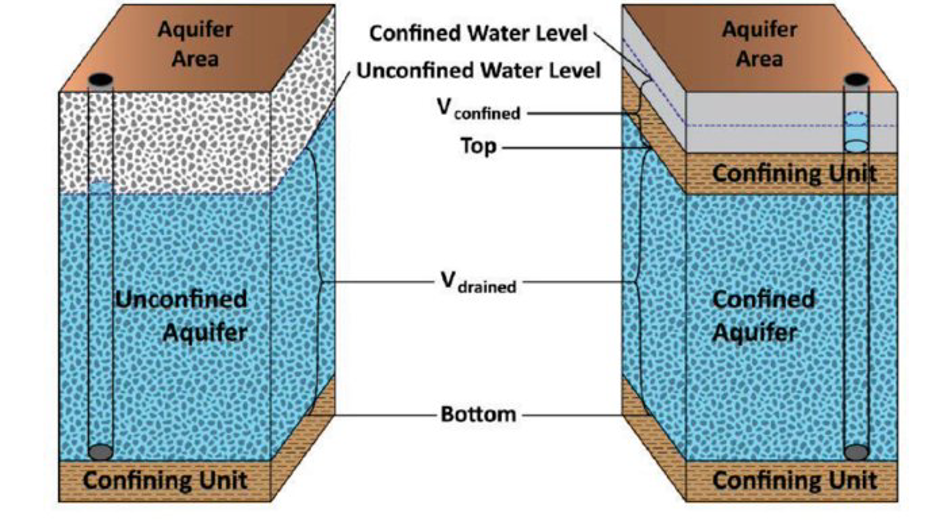
\includegraphics[width=0.95\linewidth]{figures/figures theory/Jones et al.png}
    \caption{Schematic graph of an unconfined (left) and confined aquifer (right) \cite{jones-2013}.}
    \label{aquifer}
\end{figure}
\noindent
The flow of water in the subsoil is a 3D-spatial process. Spatial differences in ground level height, degree of permeability of the soil, hydrological environment, relative humidity, weather conditions and precipitation, and atmospheric pressure play a significant role in the potential distribution and, in the end, the flow patterns of groundwater \cite{dufour-1998}. The groundwater level in a monitoring well can be investigated by measuring the weighted average pressure head over the entire perforated length of the well. 
The extent of measuring depends on parameters such as the type of monitoring well, soil composition and the hydrological situation. The hydrological situation in this context can be defined as: 1) Hydrostatic equilibrium; 2) Non-hydrostatic equilibrium with upward and downward seepage; 3) Stationary and non-stationary situation \cite{ritzema-2012}. The hydrostatic equilibrium can be illustrated as no movement of groundwater in the subsoil. If a monitoring well is present in the subsoil, water in the well is in hydrostatic equilibrium. The water level in the well is at a constant height and there is no pressure head gradient. While a non-hydrostatic equilibrium can be defined as water movement in the subsoil with an additional distinction between downward and upward seepage. Generally, air pressure influences the fluctuation of the groundwater well. For the quantification of measuring data with a high frequency (< 24 hours). The abstraction of soil moisture through the roots of vegetation can also influence the daily fluctuation of the groundwater level \cite{ritzema-2012}. Figure \labelcref{dufour} illustrates the hydrological situation with among others the processes of infiltration and seepage to the first and second aquifer. 

\begin{figure}[h]
    \centering
    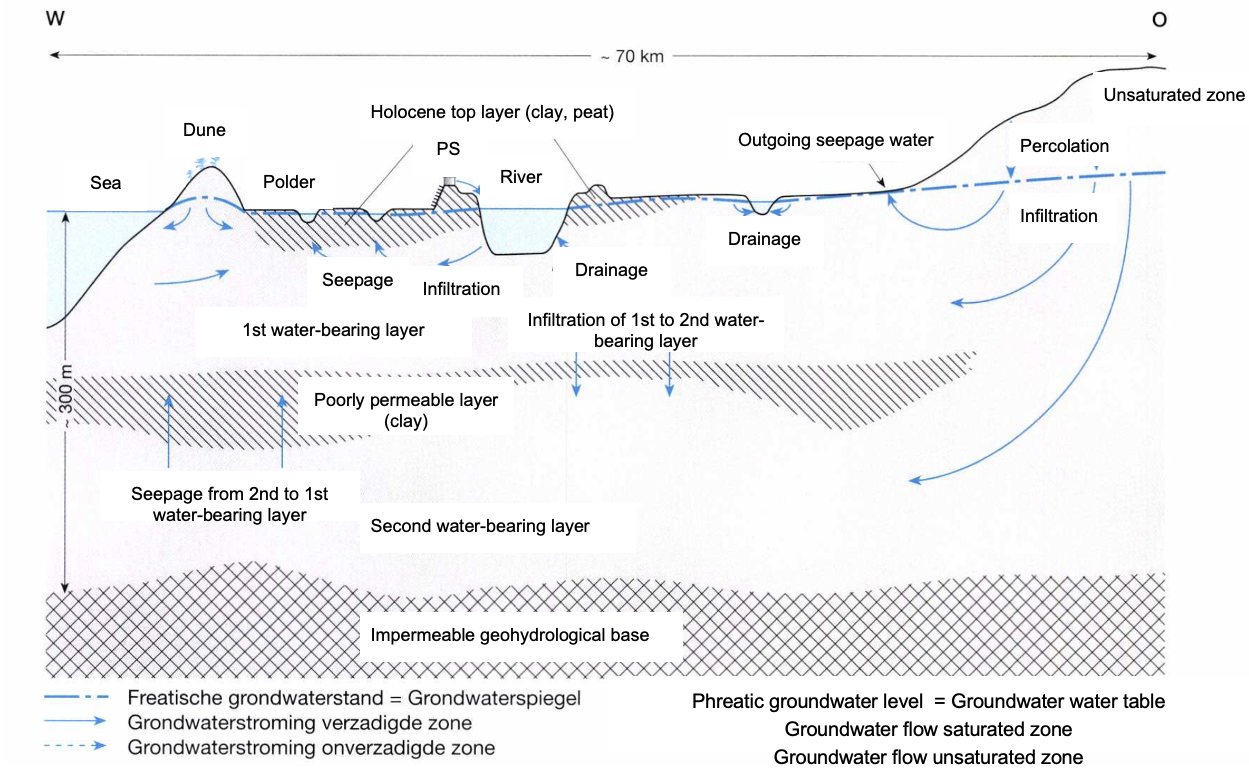
\includegraphics[width=0.95\linewidth]{figures/figures theory/dufour vertaling.png}
    \caption{Hydrological situation and process in the western part of the municipal area of Rotterdam translated, based on Dufour \cite{dufour-1998}.}
    \label{dufour}
\end{figure}
\newpage
\section{Groundwater level monitoring}
%\textit{Rotterdam’s groundwater monitoring network will be covered in this section. A general outline of the management plans and policies is presented after the description of and illustration of the current design. }
A GWMN includes a cluster of monitoring wells that are strategically placed to measure groundwater levels. The network is crucial for effective groundwater management and serves as a tool for groundwater management and, inadvertently, for integrated water management \cite{vries-1992}. A GWMN acts as a tool for gathering information about a groundwater system. A monitoring well provides information on the state of the groundwater. Single measurements nor isolated monitoring wells provide additional value, because of the spatio-temporal deviations over time, an adequate monitoring plan is required. The objective of a GWMN and the additional interests depend on local themes, this can even differ across neighborhoods in the municipal area. If groundwater nuisance is occurring, it is needed to determine the phreatic groundwater level. A GWMN can provide a prediction of the groundwater dynamics in the area. Differences between calculations and monitoring can give an indication of the quality of the model \cite{zelfde-2011}. It has to be noted that groundwater level monitoring with the use of monitoring wells is one of the essential parts of groundwater management. Yet, it is not possible to install monitoring wells at every corner of the street, but for effective groundwater management it is proven to be a prerequisite to explore the status of groundwater at 'forgotten' locations. To reduce the costs of (re)construction and installation of additional monitoring wells, it is key to identify the most appropriate locations \cite{massop-2003}. 

A potential approach for identifying a representative monitoring location in an existing network involves the computation of the parameters average groundwater level, system inertia, recharge sensitivity, which describe the groundwater dynamics together, and through field assessments \cite{massop-2003}. The existing monitoring wells are examined to determine if the well qualifies as representative. In the study by Massop and van der Gaast, the objective is not to find the most suitable monitoring location, but to assess the existing GWMN based on the representativeness and the potential for remediation and expansion \cite{massop-2003}. The result of the assessment is a set of locations that is representative for the distribution of properties that occurs within the entire research area as well as distinguished clusters to achieve a representative reflection of the variation in groundwater level [m].

\section{Groundwater management and policies} 
Groundwater management is an integrated cluster of water system management. The government, provinces, water boards and municipalities execute tasks within groundwater management. Regulating groundwater management can be divided into quantitative and qualitative groundwater management. Both quantitative and qualitative management include strategic and operational management, which comprises tasks as policy planning, framework construction, granting and enforcing  permits \cite{rws-wvl-2012}. Since 2009, the National Water Act ensures a municipal obligation of care regarding groundwater management. Although the municipality of Rotterdam is not liable for groundwater problems, they are accountable \cite{gemeente-rotterdam-no-dateA}. Important objectives in the context of groundwater policies are included in the\textit{ “Gemeentelijk Rioleringsplan”} (Municipal Sewage Plan) \cite{gemeente-rotterdam-2020B}. The Municipal Sewage Plan ensures an overview of developments that occur now and possibly can in the future within the urban water system of Rotterdam. The system consists of a sewage system, public area, and surface water system. The urban water system gathers, transports, processes, and discharges domestic wastewater, groundwater and precipitation. Within the sewage plan, there is a rough overview of what the urban system looks like, which developments are going to take place in the future, and which changes are likely to occur. Nevertheless, it is crucial to note that City of Rotterdam is not able to implement such policies by itself. Therefore, the Municipal Sewage Plan consists of three clusters: 1) The urban water system; 2) Strategy; 3) Program of the Municipal Sewage Plan of Rotterdam. The sewage plan has a valid time period of 5 years and comprises the period of 2021-2025. Within this period, the \textit{“Omgevingswet”} (National Environmental Act) was also initiated. With the start of the National Environmental Act, the Municipal Sewage Plan is not mandatory for the city anymore. Nevertheless, they choose to extend the program. Partly because of the desires of the city and its residents, but also because of the costs that are connected with the urban water system. The Municipal Sewage Plan provides insight into the expenses and justifies the municipal sewage fees \cite{gemeente-rotterdam-2020B}, as shown in figure \labelcref{MSP}. The tasks within the green boxes fall under the municipality's jurisdiction, while responsibilities like water purification, drinking water provision, and surface water management are handled by Rijkswaterstaat, water boards, and drinking water companies, respectively.
\begin{figure}[htbp]
    \centering
    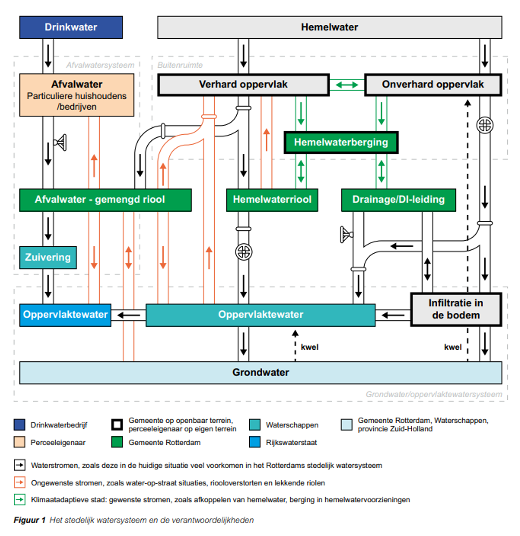
\includegraphics[width=0.75\linewidth]{figures/figures theory/rotterdam2020a.png}
    \caption{Overview of the urban water system according to the Municipal Sewage Plan of Rotterdam \cite{gemeente-rotterdam-2020A}.}
    \label{MSP}
\end{figure}

\\
